\documentclass{MastersThesis}

% ── Packages ────────────────────────────────────────────────────────────────
\usepackage{amsmath}
\usepackage{amssymb}
\usepackage{textcomp}
\usepackage{xcolor}
\usepackage{newunicodechar}
\newunicodechar{—}{\textemdash}
\newunicodechar{–}{\textendash}
\newunicodechar{§}{\S}
\newunicodechar{→}{$\rightarrow$}
\newunicodechar{✓}{\checkmark}
\newunicodechar{✗}{$\times$}
\usepackage{listings}
\usepackage{inconsolata}
\usepackage{graphicx}
\usepackage{triton}
\tritoncli{node /Volumes/Projects/triton/latex/dist/cli.cjs}
\usepackage{booktabs}
\usepackage{tabularx}
\usepackage{longtable}
\usepackage{caption}
\usepackage{fancyvrb}
\usepackage{hyperref}
\hypersetup{hidelinks}

% ── TikZ ─────────────────────────────────────────────────────────────────────
\usepackage{tikz}
\usetikzlibrary{shapes,arrows,positioning,fit,calc}

% ── Listings ────────────────────────────────────────────────────────────────
\lstset{
  basicstyle=\ttfamily\small,
  breaklines=true,
  breakatwhitespace=true,
  frame=single,
  framerule=0.5pt,
  rulecolor=\color{gray!50},
  backgroundcolor=\color{gray!5},
  numbers=left,
  numberstyle=\tiny\color{gray},
  numbersep=8pt,
  tabsize=2,
  showstringspaces=false,
  captionpos=b
}

% C++
\lstdefinelanguage{cpp}{
  morekeywords={auto,bool,break,case,catch,char,class,const,continue,default,
    delete,do,double,else,enum,explicit,extern,false,float,for,friend,goto,if,
    inline,int,long,mutable,namespace,new,noexcept,nullptr,operator,override,
    private,protected,public,return,short,signed,sizeof,static,struct,switch,
    template,this,throw,true,try,typedef,typename,union,unsigned,using,
    virtual,void,volatile,while},
  sensitive=true,
  comment=[l]{//},
  morecomment=[s]{/*}{*/},
  morestring=[b]",
  morestring=[b]'
}

% SQL
\lstdefinelanguage{sql}{
  morekeywords={SELECT,FROM,WHERE,JOIN,LEFT,RIGHT,INNER,OUTER,ON,AS,INSERT,
    INTO,VALUES,UPDATE,SET,DELETE,CREATE,TABLE,INDEX,DROP,ALTER,ADD,COLUMN,
    PRIMARY,KEY,FOREIGN,REFERENCES,UNIQUE,NOT,NULL,DEFAULT,WITH,RECURSIVE,
    ORDER,BY,GROUP,HAVING,LIMIT,OFFSET,UNION,ALL,DISTINCT,MATCH,RANK},
  sensitive=false,
  comment=[l]{--},
  morecomment=[s]{/*}{*/},
  morestring=[b]"
}

% ── Metadata ────────────────────────────────────────────────────────────────

\title{codetopo\\[0.4em]\Large A Structural Code Intelligence MCP Server\\[0.3em]\normalsize Architecture \& Design}
\author{codetopo Project}
\date{June 2026}

% ── Document ────────────────────────────────────────────────────────────────
\begin{document}
\maketitle

\begin{quote}\small
\textbf{Scope of this document.} This document describes codetopo \emph{as it
is implemented and designed}. It covers the indexing pipeline, the symbol graph
data model, the multi-root workspace design, the query engine, and the MCP
protocol surface. Features that are not yet built are listed explicitly in
\S\ref{sec:status}, not described as if they were. The document is intended to
serve as both a design reference and an onboarding guide for contributors.
\end{quote}

\tableofcontents
\newpage

\section{Overview}
\label{sec:overview}

codetopo is a structural code intelligence MCP server for AI agents. It indexes
source trees with tree-sitter~\cite{brunsfeld2018treesitter}, builds a persistent
symbol graph in SQLite, and exposes that graph to language models and developer
<<<<<<< HEAD
tools through the Model Context Protocol~\cite{anthropic2024mcp}.\footnote{MCP was publicly announced at Anthropic's developer day in November 2024. The protocol version string \texttt{2024-11-05} reflects this origin date; MCP versions are identified by calendar date.}
=======
tools through the Model Context Protocol~\cite{anthropic2024mcp}.
>>>>>>> origin/main

\subsection{The central claim}

Language models that navigate codebases today overwhelmingly rely on text
search: grep-style substring matching or embedding-vector approximate retrieval.
Both approaches treat source code as a bag of tokens. codetopo takes a
different stance: source code has \emph{structure}, and that structure---the
symbol graph---is the right primary index.

A symbol graph records what symbols exist (\emph{nodes}: functions, classes,
variables, types), how they relate (\emph{edges}: calls, imports, inheritance,
field access), and where they live (\emph{location}: file, line, column). Given
a symbol graph an LLM can answer questions that text search cannot:
``what calls \texttt{parse\_expr}?'', ``what does \texttt{Widget} inherit from?'',
``what symbols does \texttt{server.cpp} export?'' --- in milliseconds, without
reading source files. Figure~\ref{fig:symbol-graph} shows the scale of graph
that codetopo treats as its fundamental unit of navigation.

\begin{figure}[htbp]
  \centering
  \tritonnext{width=0.78\textwidth}
\begin{triton}
nodegraph
  directed
  title Tiny codetopo symbol graph
  node IDX : index_file()
  node PAR : parse_file()
  node INS : insert_batch()
  node SRV : mcp_server()
  IDX -> PAR : calls
  IDX -> INS : writes
  SRV -> IDX : imports
\end{triton}
  \caption{A small codetopo symbol graph with symbol nodes and labeled call,
           import, and write edges.}
  \label{fig:symbol-graph}
\end{figure}

\subsection{The problem it solves}

Current LLM-assisted coding tools face a fundamental tension: context windows
are finite, but codebases are large. The standard response is to retrieve
snippets by embedding similarity. This works for local, semantic queries but
fails for structural ones. A call-graph traversal expressed as a text search
requires the model to read every file that might contain a call; with codetopo
the traversal is a single SQL join.

codetopo shifts the \emph{navigation burden} from the model to the index.
The model asks a precise structural question (``give me the callers of
\texttt{foo} up to depth~3'') and receives a compact, structured answer. It
never needs to load intermediate files. This design is motivated by empirical
findings on how developers navigate large codebases~\cite{robillard2004codenav}.

\subsection{Design properties}

\begin{description}
  \item[Structural-first.] The primary index is a symbol graph, not a text
        corpus. Full-text search is provided as a complement via an FTS5
        trigram index~\cite{hipp2014fts5}, not as a substitute.
  \item[Zero-dependency runtime.] The MCP server is a single compiled binary;
        the index is a single SQLite file. No language server, no daemon, no
        network service is required.
  \item[Polyglot.] Thirteen languages are supported out of the box: C, C++,
        C\#, TypeScript, JavaScript, Python, Rust, Java, Go, Bash, SQL, and
<<<<<<< HEAD
        YAML.\footnote{Lua is the thirteenth language; it is tracked as
        experimental and omitted from this list. Simon's architecture notes
        enumerate twelve production-ready languages.} Any language with a
        tree-sitter grammar can be added with a thin extractor.
=======
        YAML. Any language with a tree-sitter grammar can be added with a
        thin extractor.
>>>>>>> origin/main
  \item[Multi-root.] A single server instance manages multiple workspace
        roots simultaneously (\S\ref{sec:workspace}).
  \item[Incremental.] Files are re-indexed only when their content changes
        (mtime $+$ xxHash check). A filesystem watcher triggers live
        re-indexing on create, modify, and delete events.
  \item[MCP-native.] codetopo speaks the Model Context Protocol
        (\S\ref{sec:mcp-protocol}) natively: JSON-RPC~2.0 over stdio, the
<<<<<<< HEAD
        same transport as         the Language Server Protocol~\cite{microsoft2016lsp}\footnote{LSP was
        first announced by Microsoft and Red Hat on June~27, 2016 ---
        coincidentally the same calendar date as this document's writing.}
=======
        same transport as the Language Server Protocol~\cite{microsoft2016lsp}
>>>>>>> origin/main
        but with a tool-call interface designed for autonomous agents.
\end{description}

\subsection{What codetopo is not}

codetopo is a code intelligence \emph{index and query server}. It does
\emph{not} compile code, does \emph{not} run tests, does \emph{not} generate
code, and does \emph{not} replace a full language server. It provides the
structural substrate on which tools and agents can build.

\section{Architecture}
\label{sec:architecture}

codetopo is organized into four layers: Indexer, Storage, Query Engine, and
MCP Server. Each layer has a single responsibility and communicates with
adjacent layers through a narrow interface.

\begin{figure}[htbp]
\centering
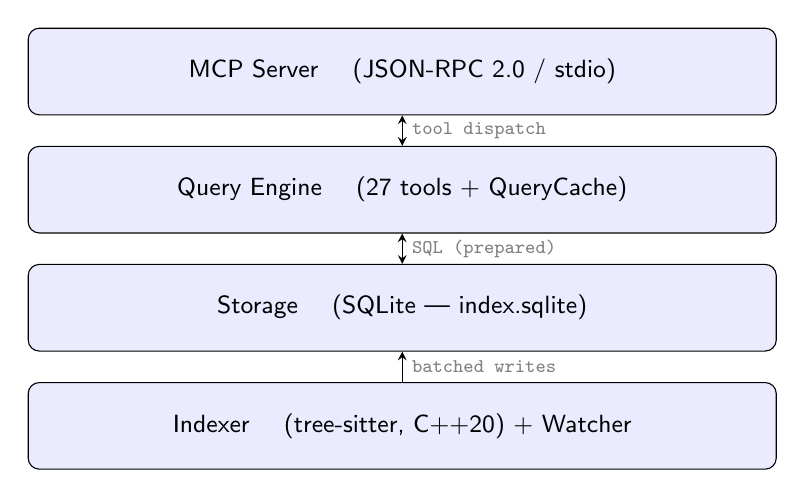
\begin{tikzpicture}[
  layer/.style={draw, fill=blue!8, rounded corners,
                minimum width=9.5cm, minimum height=1.1cm, text centered,
                font=\small\sffamily},
  ann/.style={font=\scriptsize\ttfamily, text=gray},
  >=stealth
]
\node[layer] (mcp)     at (0,4.5) {MCP Server \quad (JSON-RPC 2.0 / stdio)};
\node[layer] (query)   at (0,3.0) {Query Engine \quad (27 tools + QueryCache)};
\node[layer] (storage) at (0,1.5) {Storage \quad (SQLite --- index.sqlite)};
\node[layer] (indexer) at (0,0.0) {Indexer \quad (tree-sitter, C++20) + Watcher};

\draw[<->] (mcp)     -- (query)   node[ann,right,midway] {tool dispatch};
\draw[<->] (query)   -- (storage) node[ann,right,midway] {SQL (prepared)};
\draw[->]  (indexer) -- (storage) node[ann,right,midway] {batched writes};
\end{tikzpicture}
\caption{codetopo four-layer architecture.}
\label{fig:architecture}
\end{figure}

\subsection{Indexer}

The Indexer scans workspace roots, parses each source file with a tree-sitter
grammar~\cite{brunsfeld2018treesitter} appropriate for its language, and
extracts symbols and edges. It writes to the Storage layer in batches within a
single SQLite transaction per file. The Indexer runs at startup (governed by a
\emph{freshness policy}: \texttt{eager}, \texttt{normal}, \texttt{lazy}, or
\texttt{off}) and on demand via the \texttt{reindex} tool.

A platform-native filesystem \emph{watcher} (FSEvents on macOS,
inotify on Linux, ReadDirectoryChangesW on Windows) monitors each workspace
root. On a create, modify, or delete event the watcher schedules an incremental
re-index of the affected file. A branch-switch event (detected by watching
\texttt{.git/HEAD}) triggers re-indexing of all files whose content has changed
since the previous HEAD.

\subsection{Storage}

Storage is a single SQLite database file (\texttt{.codetopo/index.sqlite})
co-located with or near the server binary. It holds the symbol graph, file
metadata, workspace roots, and FTS indexes. The schema is described in detail
in \S\ref{sec:data-model}. SQLite WAL mode allows the Query Engine to serve
reads while the Indexer is writing.

\subsection{Query Engine}

The Query Engine exposes 27 MCP tools. Each tool translates a structured
request into one or more SQL queries, formats the result, and returns it as a
JSON-RPC response. Frequently used statements are cached as \emph{prepared
statements} in a \texttt{QueryCache} keyed by tool name; the cache is
invalidated on each re-index. The tools are organized by capability and
described in \S\ref{sec:mcp-protocol}.

\subsection{MCP Server}

The MCP Server owns the JSON-RPC transport layer (stdio). It performs
protocol negotiation (handshake returns \texttt{protocolVersion 2024-11-05}),
tool registration, and request routing to the Query Engine. Staleness
detection is managed by a \texttt{StalenessState} object that tracks the
mtime of \texttt{.git/HEAD}, the indexed branch/commit, and a
\texttt{\_meta.stale} flag that is included in tool responses when the index
may be out of date.

\subsection{Data flow}

At startup the server opens the database, validates the schema (running
migrations if needed), loads workspace roots, and starts the Indexer for any
root with stale or missing index data (subject to the freshness policy). Once
indexing is complete the server enters its serve loop: it reads JSON-RPC
requests from stdin, dispatches each to the appropriate Query Engine tool via
the prepared-statement cache, and writes the response to stdout.

\section{Indexing Pipeline}
\label{sec:indexing-pipeline}

The indexing pipeline transforms a directory tree of source files into the
symbol graph stored in SQLite~\cite{brunsfeld2018treesitter}. It runs in five
stages organized into two phases: a structural phase that builds the symbol
graph and a deferred FTS phase that populates the content index.

\begin{figure}[htbp]
\centering
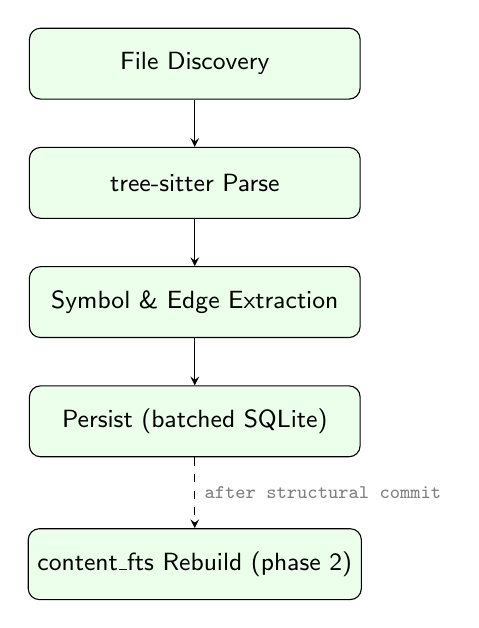
\begin{tikzpicture}[
  box/.style={draw, fill=green!8, rounded corners,
              minimum width=4.2cm, minimum height=0.9cm,
              text centered, font=\small\sffamily},
  phase/.style={draw=gray, dashed, rounded corners, inner sep=6pt},
  ann/.style={font=\scriptsize\ttfamily, text=gray},
  >=stealth, node distance=0.6cm
]
\node[box] (discover)  {File Discovery};
\node[box] (parse)     [below=of discover]  {tree-sitter Parse};
\node[box] (extract)   [below=of parse]     {Symbol \& Edge Extraction};
\node[box] (persist)   [below=of extract]   {Persist (batched SQLite)};
\node[box] (fts)       [below=0.9cm of persist]   {content\_fts Rebuild (phase 2)};

\draw[->] (discover) -- (parse);
\draw[->] (parse)    -- (extract);
\draw[->] (extract)  -- (persist);
\draw[->, dashed] (persist) -- (fts)
  node[ann, right, midway] {after structural commit};
\end{tikzpicture}
\caption{The codetopo indexing pipeline. FTS population is deferred to phase 2
         after the structural commit to avoid holding a write lock during
         content hashing.}
\label{fig:pipeline}
\end{figure}

\subsection{File discovery}

The pipeline begins by enumerating candidate files. When the workspace root
contains a \texttt{.git} directory, codetopo prefers \texttt{git ls-files} to
enumerate tracked files; this automatically respects \texttt{.gitignore} rules
and avoids scanning build artifacts. When no Git repository is detected, the
pipeline falls back to a recursive directory walk using the embedded
\texttt{.gitignore}-aware walker. Files are filtered by extension against the
registered set of language grammars.

Each candidate file is checked against its stored \texttt{mtime} and xxHash
fingerprint. If both match the stored values, the file is skipped entirely
(no parse, no write). This incremental check is the primary source of
startup-time savings on large repositories.

\subsection{Supported languages}

The following 13 languages are supported via tree-sitter grammars and
language-specific extractors: C, C++, C\#, TypeScript, JavaScript, Python,
Rust, Java, Go, Bash, SQL, YAML, and Lua.\footnote{Simon's architecture
summary lists 12; Lua is tracked as experimental.}

\subsection{Parsing}

Accepted files are parsed with the tree-sitter grammar for their detected
language (\texttt{src/index/parser.h:30--101}). Tree-sitter produces a
concrete syntax tree (CST) in memory. Parse errors are tolerated:
tree-sitter performs error-recovery and returns partial trees for files with
syntax errors. The CST is the input to the extractor.

\subsection{Symbol and edge extraction}

The extractor (\texttt{src/index/extractor.cpp:207--297}) walks the CST using
an \emph{iterative stack-based DFS} rather than recursion. This avoids stack
overflow on deeply nested ASTs (e.g., generated files with thousands of nested
expressions).

For each traversed node the extractor identifies:
\begin{itemize}
  \item \textbf{Symbol definitions}: functions, methods, classes, structs,
        enums, type aliases, variables, and constants. Each definition
        produces a \texttt{nodes} row with kind, name, qualified name,
        signature, source span, visibility, and optional docstring.
  \item \textbf{Call expressions}: recorded as \texttt{edges} of kind
        \texttt{calls}. Where the callee can be resolved to a known symbol
        in the current or previously indexed root, the edge carries both
        \texttt{src\_id} and \texttt{dst\_id}; unresolved calls carry
        \texttt{dst\_name} only and are flagged as approximate. A confidence
        floor of 0.3 is applied: edges below that threshold are discarded.
  \item \textbf{References}: import/include, inheritance, field access, and
        type references are recorded in the \texttt{refs} table.
\end{itemize}

\subsection{Persistence}

Extracted symbols, edges, and references are written to SQLite in
\emph{batched inserts} (\texttt{src/index/persister.h:117--380}):
\begin{itemize}
  \item Symbol (node) batch size: 100 rows per statement.
  \item Reference batch size: 80 rows per statement.
  \item Edge batch size: 150 rows per statement.
\end{itemize}

Before inserting, existing rows for the file are deleted
(\texttt{DELETE WHERE file\_id = ?}), so the operation is idempotent. The
entire insert sequence for one file runs inside a single transaction.

\paragraph{Bulk mode.} When the initial index covers more than 1\,000 files,
the pipeline enters \emph{bulk mode}: it drops secondary indexes and FTS
triggers before the load and rebuilds them afterwards. This avoids repeated
B-tree rebalancing during the insert flood and significantly reduces total
indexing time on large repositories.

\subsection{FTS rebuild (phase 2)}

After the structural commit (nodes, edges, refs) is finalized, the pipeline
runs a second phase that populates \texttt{content\_fts}. This table is a
\emph{contentless} FTS5 trigram index over source lines
(\S\ref{sec:data-model}). Because it is contentless, rows cannot be copied
from another database; they must be inserted by reading source files from
disk line-by-line. Deferring this phase means the write lock is held for only
as long as the structural data requires.

\section{Data Model}
\label{sec:data-model}

The codetopo database schema consists of six principal tables and three FTS
virtual tables. This section describes each table, the relationships between
them, and the FTS indexing strategy~\cite{hipp2014fts5}.

\begin{figure}[htbp]
\centering
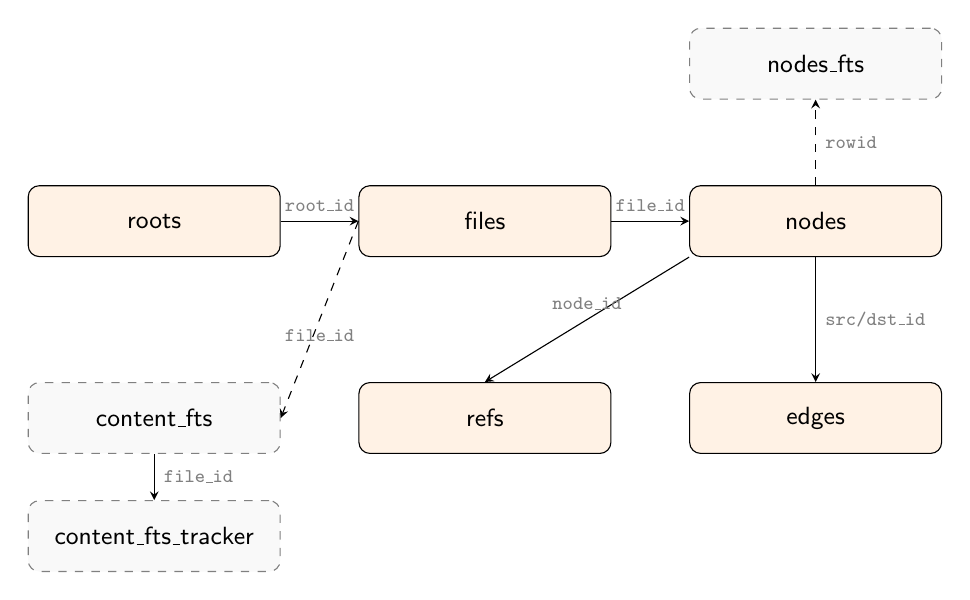
\begin{tikzpicture}[
  entity/.style={draw, fill=orange!10, rounded corners,
                 minimum width=3.2cm, minimum height=0.9cm,
                 text centered, font=\small\sffamily},
  fts/.style={draw=gray, dashed, fill=gray!5, rounded corners,
              minimum width=3.2cm, minimum height=0.9cm,
              text centered, font=\small\sffamily},
  attr/.style={font=\scriptsize\ttfamily, text=gray},
  >=stealth
]
\node[entity] (roots)   at (-4.2, 0)   {roots};
\node[entity] (files)   at ( 0,   0)   {files};
\node[entity] (nodes)   at ( 4.2, 0)   {nodes};
\node[entity] (edges)   at ( 4.2,-2.5) {edges};
\node[entity] (refs)    at ( 0,  -2.5) {refs};
\node[fts]    (nfts)    at ( 4.2, 2.0) {nodes\_fts};
\node[fts]    (cfts)    at (-4.2,-2.5) {content\_fts};
\node[fts]    (ctrk)    at (-4.2,-4.0) {content\_fts\_tracker};

\draw[->] (roots)  -- node[attr,above]{\scriptsize root\_id} (files);
\draw[->] (files)  -- node[attr,above]{\scriptsize file\_id} (nodes);
\draw[->] (nodes.south) -- node[attr,right]{\scriptsize src/dst\_id} (edges.north);
\draw[->] (nodes.south west) -- node[attr,above]{\scriptsize node\_id} (refs.north);
\draw[->, dashed] (nodes.north) -- node[attr,right]{\scriptsize rowid} (nfts.south);
\draw[->, dashed] (files.west)  -- node[attr,below]{\scriptsize file\_id} (cfts.east);
\draw[->] (cfts.south) -- node[attr,right]{\scriptsize file\_id} (ctrk.north);
\end{tikzpicture}
\caption{Entity-relationship overview of the codetopo schema. Dashed arrows
         indicate FTS virtual-table relationships.}
\label{fig:schema}
\end{figure}

\subsection{roots}

\begin{lstlisting}[language=sql]
CREATE TABLE roots (
  id       INTEGER PRIMARY KEY,
  path     TEXT    NOT NULL UNIQUE,  -- absolute, canonical path
  added_at INTEGER NOT NULL          -- Unix timestamp
);
\end{lstlisting}

Each row represents a workspace root. The \texttt{id} is used as the root
offset in the ID allocation scheme described in \S\ref{sec:workspace}.

In addition to the relational tables, the schema keeps build and repository
metadata in a small \texttt{kv} store accessed through
\texttt{set\_kv()}/\texttt{get\_kv()}; Figure~\ref{fig:schema-kv} sketches
representative entries.

\begin{figure}[htbp]
  \centering
  \tritonnext{width=0.82\textwidth}
\begin{triton}
hashmap
  title schema kv
  buckets 5
  bucket 0: schema_version->8
  bucket 1: indexer_version->2026.06, last_index_time->2026-06-28T12:48
  bucket 2: repo_root->workspace, language_coverage->13langs
  bucket 3: git_head->abc1234, git_branch->main
\end{triton}
  \caption{Representative \texttt{kv} metadata entries stored alongside the
           structural tables.}
  \label{fig:schema-kv}
\end{figure}

\subsection{files}

\begin{lstlisting}[language=sql]
CREATE TABLE files (
  id        INTEGER PRIMARY KEY,
  path      TEXT    NOT NULL,        -- path relative to root
  language  TEXT,
  root_id   INTEGER NOT NULL REFERENCES roots(id)
);
\end{lstlisting}

\subsection{nodes}

The \texttt{nodes} table stores both file-level nodes (\texttt{node\_type =
'file'}) and symbol-level nodes (\texttt{node\_type = 'symbol'}):

\begin{lstlisting}[language=sql]
CREATE TABLE nodes (
  id            INTEGER PRIMARY KEY,
  file_id       INTEGER NOT NULL REFERENCES files(id),
  node_type     TEXT    NOT NULL,   -- 'file' | 'symbol'
  kind          TEXT,               -- function|class|method|...
  name          TEXT,
  qualname      TEXT,               -- fully-qualified name
  signature     TEXT,
  span          TEXT,               -- "start_line:start_col-end_line:end_col"
  is_definition INTEGER DEFAULT 1,
  visibility    TEXT,               -- public|private|protected|...
  doc           TEXT,               -- leading docstring
  stable_key    TEXT                -- language-specific stable identifier
);
\end{lstlisting}

\subsubsection{Symbol kinds}

The \texttt{kind} field takes one of: \texttt{function}, \texttt{method},
\texttt{class}, \texttt{struct}, \texttt{enum}, \texttt{enum\_variant},
\texttt{type\_alias}, \texttt{interface}, \texttt{trait}, \texttt{variable},
\texttt{constant}, \texttt{module}, \texttt{namespace}, \texttt{macro}.

\subsection{edges}

\begin{lstlisting}[language=sql]
CREATE TABLE edges (
  id         INTEGER PRIMARY KEY,
  src_id     INTEGER REFERENCES nodes(id),
  dst_id     INTEGER REFERENCES nodes(id),
  dst_name   TEXT,     -- unresolved callee name (approx edges)
  kind       TEXT NOT NULL,
  file_id    INTEGER REFERENCES files(id),
  confidence REAL DEFAULT 1.0
);
\end{lstlisting}

Edges with \texttt{confidence} below 0.3 are discarded at extraction time.

\subsubsection{Edge kinds}

\begin{description}
  \item[\texttt{calls}] A function or method call from \texttt{src} to \texttt{dst}.
  \item[\texttt{includes}] A module import or \texttt{\#include}.
  \item[\texttt{inherits}] A class or struct extending or implementing another.
  \item[\texttt{references}] A general reference that does not fit a more
        specific kind.
  \item[\texttt{contains}] A structural containment edge (e.g., method
        contained in a class).
\end{description}

\subsection{refs}

The \texttt{refs} table records finer-grained reference sites than edges:

\begin{lstlisting}[language=sql]
CREATE TABLE refs (
  id      INTEGER PRIMARY KEY,
  node_id INTEGER REFERENCES nodes(id),
  kind    TEXT NOT NULL,
  file_id INTEGER REFERENCES files(id),
  span    TEXT
);
\end{lstlisting}

Reference kinds: \texttt{call}, \texttt{type\_ref}, \texttt{include},
\texttt{inherit}, \texttt{field\_access}, \texttt{other}.

\subsection{FTS indexes}

Three FTS-related tables are maintained~\cite{hipp2014fts5}:

\paragraph{nodes\_fts.}  A standard FTS5 content-shadow table over the
\texttt{nodes} table:

\begin{lstlisting}[language=sql]
CREATE VIRTUAL TABLE nodes_fts USING fts5(
  name, qualname, signature, doc,
  content='nodes', content_rowid='id'
);
\end{lstlisting}

This is used by \texttt{symbol\_search} for BM25-ranked prefix queries over
symbol names, qualified names, signatures, and docstrings.

\paragraph{content\_fts.}  A \emph{contentless}\footnote{A \texttt{content=}
FTS5 table mirrors the original rows in its shadow tables, enabling
snippet generation from stored data, but it doubles storage --- every indexed
string is kept both in the shadow table and on disk. The contentless variant
(\texttt{content=''}) stores only the inverted index, halving storage at the
cost of requiring the source file to be re-read for result display. This
trade-off is acceptable because source files are always present locally.}
FTS5 table with the trigram
tokenizer, indexed per source line:

\begin{lstlisting}[language=sql]
CREATE VIRTUAL TABLE content_fts USING fts5(
  line_text,
  file_id UNINDEXED,
  line_no  UNINDEXED,
  content='',
  tokenize='trigram'
);
\end{lstlisting}

Because this table is contentless (it does not store the original text),
it cannot be scanned for its row contents. Results are retrieved by matching
on \texttt{line\_text} and then reading the actual source from disk.

\paragraph{content\_fts\_tracker.}  A plain table that tracks which files
have been indexed into \texttt{content\_fts}, since the FTS table itself
cannot be queried for its file coverage:

\begin{lstlisting}[language=sql]
CREATE TABLE content_fts_tracker (
  file_id INTEGER PRIMARY KEY REFERENCES files(id)
);
\end{lstlisting}

\subsection{Multi-root ID scheme}

All nodes across all workspace roots share a single \texttt{nodes} table. To
keep IDs globally unique, codetopo uses a multiplicative offset\footnote{The
factor $10^9$ was chosen for readability in debug output: root 1's IDs begin
at \texttt{1\,000\,000\,001}. SQLite's 64-bit signed rowid ceiling
($2^{63}-1 \approx 9.2 \times 10^{18}$) accommodates up to $\sim$9.2 billion
root slots at this scale, far beyond any practical need.}:
\[
  \text{global\_id} = \text{root\_id} \times 10^9 + \text{local\_id}
\]
where \texttt{local\_id} is the SQLite autoincrement rowid within the root's
ID space ($1$ through $10^9 - 1$). This scheme supports up to $10^9 - 1$
symbols per root. The full scheme is described in \S\ref{sec:workspace}.

\section{MCP Protocol}
\label{sec:mcp-protocol}

\subsection{Background}

The Model Context Protocol~\cite{anthropic2024mcp} is an open JSON-RPC~2.0
protocol, inspired by the Language Server Protocol~\cite{microsoft2016lsp},
designed for connecting LLM applications to external data sources and tools.
Like LSP, it runs over stdio with newline-delimited JSON messages. Unlike LSP
(which is editor-to-language-server), MCP is agent-to-tool-server: the
client is an LLM or AI agent, and the server exposes \emph{tools} --- named
callable operations with typed input schemas.

\subsection{Why MCP for code intelligence}

The tool-call pattern maps naturally to code intelligence queries. An AI agent
can call \texttt{symbol\_search} as naturally as it calls any other function.
The structured JSON input/output means the agent never needs to parse
grep-style output or interpret editor hover text. codetopo registers 27 tools
that cover the full range of structural queries an AI agent needs when
working on a codebase.

\subsection{Transport and framing}

\begin{itemize}
  \item Transport: stdio (one server process per client session).
  \item Framing: newline-delimited JSON (NDJSON); each message is a UTF-8
        JSON object terminated by \verb|\n|.
  \item Protocol version: \texttt{2024-11-05}\footnote{MCP protocol versions
        use calendar-date strings. \texttt{2024-11-05} is the version at which
        the core tool-call, prompts, and resources primitives were stabilized
        in the initial public specification.} (returned in the handshake
        \texttt{initialize} response).
\end{itemize}

\subsection{Connection lifecycle}

\begin{enumerate}
  \item Client sends \texttt{initialize} with protocol version and
        client capabilities.
  \item Server responds with \texttt{protocolVersion}, server info, and the
        full tool list.
  \item Client sends \texttt{initialized} notification.
  \item Client sends \texttt{tools/call} requests; server responds with results.
  \item Either side may send \texttt{shutdown} to end the session.
\end{enumerate}

\subsection{Staleness detection}

Each tool response includes a \texttt{\_meta} object. When the server detects
that the index may be out of date --- by checking the mtime of
\texttt{.git/HEAD} against the timestamp of the last index run --- it sets
\texttt{\_meta.stale = true}. Clients should treat stale responses as advisory:
the data is the last known good state, but a call to \texttt{reindex} is
recommended.

\subsection{QueryCache}

The \texttt{QueryCache} is an in-process prepared-statement cache keyed by
tool name. Preparing a SQLite statement compiles it to bytecode; caching avoids
re-compilation on every tool call. The cache is cleared (all statements
finalized) at the start of each re-index cycle so that schema changes take
effect immediately.

\subsection{Tool catalogue}

The 27 tools are organized into eight categories.

\subsubsection{Navigation}

\begin{description}
  \item[\texttt{dir\_list}] List files and directories under a path.
  \item[\texttt{file\_search}] Find files by name pattern across all roots.
  \item[\texttt{file\_summary}] Return symbol-annotated outline of a file.
  \item[\texttt{source\_at}] Read raw source content at a given path.
\end{description}

\subsubsection{Symbol lookup}

\begin{description}
  \item[\texttt{symbol\_search}] FTS5 prefix search over symbol names,
        qualified names, signatures, and docstrings. \texttt{kind='function'}
        matches both \texttt{function} and \texttt{method} nodes for
        polyglot parity.
  \item[\texttt{symbol\_list}] List all symbols of a given kind in a root.
  \item[\texttt{symbol\_get}] Fetch a single symbol by ID.
  \item[\texttt{symbol\_get\_batch}] Fetch multiple symbols by ID in one
        round-trip.
\end{description}

\subsubsection{Graph traversal}

\begin{description}
  \item[\texttt{callers\_approx}] Direct callers of a symbol (inbound
        \texttt{calls} edges). Named ``approx'' because call edges are
        AST-derived without full type resolution.
  \item[\texttt{callees\_approx}] Direct callees of a symbol (outbound
        \texttt{calls} edges), including unresolved name-only entries.
  \item[\texttt{references}] All reference sites for a symbol across all roots.
  \item[\texttt{context\_for}] Return the symbol context (enclosing function
        or class) for a given file location.
  \item[\texttt{entrypoints}] Identify symbols with no callers (potential
        entry points or public API).
\end{description}

\subsubsection{Impact analysis}

\begin{description}
  \item[\texttt{impact\_of}] Transitive BFS/DFS over the call graph from a
        seed node; returns all symbols reachable via \texttt{calls} edges.
  \item[\texttt{subgraph}] Extract the subgraph reachable from a set of seed
        nodes up to a given depth.
  \item[\texttt{shortest\_path}] Find the shortest call path between two
        symbols using BFS.
  \item[\texttt{dependency\_cluster}] Group symbols by mutual dependency into
        clusters.
  \item[\texttt{find\_implementations}] Find concrete implementations of an
        interface, trait, or abstract method.
\end{description}

Figure~\ref{fig:dependency-clusters} illustrates the partitioned output shape
of \texttt{dependency\_cluster}: symbols that share strong mutual dependencies
collapse into the same set.

\begin{figure}[htbp]
  \centering
  \tritonnext{width=0.68\textwidth}
\begin{triton}
unionfind 7
  title dependency clusters
  parent 0 0 1 3 3 5 5
\end{triton}
  \caption{A disjoint-set view of \texttt{dependency\_cluster} output, where
           each connected group is a coupled symbol cluster.}
  \label{fig:dependency-clusters}
\end{figure}

\subsubsection{Metadata}

\begin{description}
  \item[\texttt{repo\_stats}] Row counts, language distribution, and index
        size.
  \item[\texttt{server\_info}] Server version, protocol version, and
        supported languages.
  \item[\texttt{reindex}] Trigger an incremental or full re-index of all roots.
\end{description}

\subsubsection{File analysis}

\begin{description}
  \item[\texttt{file\_deps}] Return the import/include dependency graph for a
        file.
  \item[\texttt{method\_fields}] List the fields accessed by a method (field
        access edges).
\end{description}

\subsubsection{Workspace management}

\begin{description}
  \item[\texttt{workspace\_add}] Add a new root path to the workspace.
  \item[\texttt{workspace\_remove}] Remove a root and cascade-delete its data.
  \item[\texttt{workspace\_list}] List all registered roots with status and
        statistics.
\end{description}

\subsubsection{Full-text search}

\begin{description}
  \item[\texttt{code\_search}] Trigram full-text search over source lines
        using the \texttt{content\_fts} contentless FTS5 index~\cite{cox2012trigram}.
        Returns matching lines with file path and line number.
\end{description}

\section{Multi-Root Workspace}
\label{sec:workspace}

\subsection{Problem}

A developer working on a project often needs to navigate \emph{reference
codebases} alongside their main project: a dependency's source, a shared
library, or a related service. codetopo supports this via \emph{workspace
roots}: named, absolute filesystem paths that are all indexed and queryable
within a single server instance.

\subsection{Design}

All roots share a single \texttt{index.sqlite} database with no mode
switching. The \texttt{roots} table (\S\ref{sec:data-model}) maps each root
to an integer ID; the \texttt{files} table records \texttt{root\_id} on every
file row. There is no separate per-root database.

\subsection{ID offset scheme}

Nodes, files, and edges across all roots share a single ID space. codetopo
ensures uniqueness with a multiplicative offset:

\[
  \text{global\_id} = \text{root\_id} \times 10^9 + \text{local\_id}
\]

\texttt{local\_id} is the SQLite autoincrement rowid within the root's space
(values $1$ through $10^9 - 1$). A signed 64-bit integer ($\approx 9.2 \times
10^{18}$) supports around 9 billion root-slots at this scale, far beyond any
practical need. Because all IDs are stored in a single file, no cross-root
join is needed: a node ID uniquely identifies both the root and the local
record. Figure~\ref{fig:id-offset-array} visualizes one root-local slot before
the offset formula lifts it into the global ID space.

\begin{figure}[htbp]
  \centering
  \tritonnext{width=0.7\textwidth}
\begin{triton}
array
  title local_id within one root slot
  cells 1 2 3 4 5
  index
  ptr local_id -> 2
\end{triton}
  \caption{A root-local ID slot before conversion into the global
           \texttt{root\_id * 10\^{}9 + local\_id} namespace.}
  \label{fig:id-offset-array}
\end{figure}

\subsection{Path handling}

All paths stored in the database are \emph{relative to their root}. Tools that
accept filesystem paths call \texttt{resolve\_db\_path()}, which tries three
strategies in order:
\begin{enumerate}
  \item Absolute path match: \texttt{root.path || '/' || file.path = :abs}.
  \item Exact relative match against \texttt{files.path}.
  \item Suffix \texttt{LIKE} match: \texttt{files.path LIKE '\%' || :suffix}.
\end{enumerate}
The suffix match handles editors that pass workspace-relative paths without
specifying the root. This approach is necessary because workspace roots may
live at different absolute paths on different machines.

\subsection{Workspace operations}

\subsubsection{Adding a root}

\texttt{workspace\_add} accepts an absolute path. The flow is:
\begin{enumerate}
  \item Canonicalize the path (resolve symlinks).
  \item Ensure the path is indexed: if no \texttt{roots} row exists, run a
        full index first.
<<<<<<< HEAD
  \item \texttt{ATTACH} the source database (if separate).\footnote{A SQLite
        gotcha: \texttt{ATTACH DATABASE} must be issued \emph{before}
        \texttt{BEGIN TRANSACTION} on the same connection. Attempting to
        attach inside an open transaction raises \texttt{SQLITE\_ERROR}. The
        workspace-add flow therefore attaches the source database first, then
        opens the write transaction for the row copy.}
=======
  \item \texttt{ATTACH} the source database (if separate).
>>>>>>> origin/main
  \item \texttt{INSERT} a row into \texttt{roots} to obtain the new
        \texttt{root\_id}.
  \item Copy all \texttt{files}, \texttt{nodes}, \texttt{edges}, and
        \texttt{refs} rows, re-keying IDs using the offset formula.
  \item Rebuild \texttt{content\_fts} from disk (line by line per file),
        because contentless FTS tables cannot be copied directly.
\end{enumerate}

\subsubsection{Removing a root}

\texttt{workspace\_remove} runs:
\begin{enumerate}
  \item Delete \texttt{content\_fts} rows for the root's files.
  \item \texttt{DELETE FROM roots WHERE id = :root\_id}.
  \item Foreign-key cascades remove dependent rows in \texttt{files},
        \texttt{nodes}, \texttt{edges}, and \texttt{refs}.
\end{enumerate}
The entire operation runs in a single transaction.

\subsubsection{Listing roots}

\texttt{workspace\_list} returns all roots with path, symbol count, file
count, last-indexed timestamp, and indexing status.

\subsection{Indexer guard}

The normal \texttt{codetopo index} command only re-indexes files belonging to
the main project (\texttt{files.root\_id IS NULL} or the root with
\texttt{id = 0}). It does not overwrite data for workspace roots added via
\texttt{workspace\_add}. This prevents accidental resets of externally indexed
roots.

\subsection{Concurrent access}

SQLite WAL mode allows the Query Engine to serve reads while the Indexer is
writing. The Indexer acquires a write lock only during the commit phase of each
file transaction; reads proceed unblocked during parse and extraction.

\section{Query Engine}
\label{sec:query-engine}

The Query Engine translates structured MCP tool requests into SQL queries
against the symbol graph. This section describes the major query patterns.
Motivation for tool-based code navigation is grounded in empirical studies of
how developers investigate large codebases~\cite{robillard2004codenav}.

\subsection{Symbol search}

\texttt{symbol\_search} queries the \texttt{nodes\_fts} FTS5 virtual table
(\S\ref{sec:data-model}) with a prefix \texttt{MATCH} on the \texttt{name}
column:

\begin{lstlisting}[language=sql]
SELECT n.id, n.name, n.qualname, n.kind, f.path, n.span
FROM   nodes n
JOIN   files f ON f.id = n.file_id
JOIN   nodes_fts nf ON nf.rowid = n.id
WHERE  nf.name MATCH :query || '*'
  AND  n.node_type = 'symbol'
  AND  (:root_id IS NULL OR f.root_id = :root_id)
ORDER  BY rank
LIMIT  :limit;
\end{lstlisting}

A \texttt{kind='function'} filter expands to \texttt{kind IN ('function',
'method')} to achieve polyglot parity: in Python a method has kind
\texttt{method} while in C a standalone function has kind \texttt{function},
but both are callable symbols.

\subsection{Call graph traversal}
\label{sec:qe-callgraph}

Call graph construction at query time is based on edges extracted by the
indexer~\cite{ryder1979callgraph,grove2001callgraph}. Because codetopo
does not perform type resolution, these edges are AST-derived approximations
--- hence the ``approx'' suffix on the tool names.

\subsubsection{callers\_approx}

\begin{lstlisting}[language=sql]
SELECT n.id, n.name, n.kind, f.path, n.span
FROM   edges e
JOIN   nodes n ON n.id = e.src_id
JOIN   files f ON f.id = n.file_id
WHERE  e.dst_id = :node_id
  AND  e.kind   = 'calls';
\end{lstlisting}

\subsubsection{callees\_approx}

\begin{lstlisting}[language=sql]
SELECT e.dst_id, e.dst_name, n.kind, f.path, n.span
FROM   edges e
LEFT   JOIN nodes n ON n.id = e.dst_id
LEFT   JOIN files f ON f.id = n.file_id
WHERE  e.src_id = :node_id
  AND  e.kind   = 'calls';
\end{lstlisting}

When \texttt{dst\_id} is \texttt{NULL}, the callee is returned by name only
(\texttt{dst\_name}): an unresolved reference retained from the extractor.

\subsection{Impact analysis}

\texttt{impact\_of} computes the transitive closure of the call graph starting
from a seed node using a BFS/DFS over \texttt{calls} edges. A recursive
CTE expresses this efficiently in SQLite:

\begin{lstlisting}[language=sql]
WITH RECURSIVE impact(id, depth) AS (
  SELECT :seed_id, 0
  UNION ALL
  SELECT e.dst_id, i.depth + 1
  FROM   edges e
  JOIN   impact i ON e.src_id = i.id
  WHERE  e.kind = 'calls' AND i.depth < :max_depth
)
SELECT DISTINCT n.id, n.name, n.kind, f.path, i.depth
FROM   impact i
JOIN   nodes n ON n.id = i.id
JOIN   files f ON f.id = n.file_id
ORDER  BY i.depth, n.name;
\end{lstlisting}

\texttt{shortest\_path} uses a similar CTE with early termination when the
target node is reached.

\subsection{Path resolution}

\texttt{resolve\_db\_path()} converts a filesystem path into a database
\texttt{file\_id}. It tries three strategies:

\begin{enumerate}
  \item \textbf{Absolute match}: \texttt{roots.path || '/' || files.path = :abs}
  \item \textbf{Exact relative match}: \texttt{files.path = :rel}
  \item \textbf{Suffix LIKE match}: \texttt{files.path LIKE '\%' || :suffix}
\end{enumerate}

Strategy 3 handles workspace roots with absolute paths that differ between
machines, and editor integrations that pass workspace-relative paths.

\subsection{Content full-text search}

\texttt{code\_search} uses \texttt{content\_fts}, the contentless trigram FTS5
table populated per source line~\cite{cox2012trigram}:

\begin{lstlisting}[language=sql]
SELECT f.path, r.path AS root_path,
       cft.line_no,
       snippet(content_fts, 0, '', '', '...', 10) AS excerpt
FROM   content_fts
JOIN   content_fts_tracker cft USING (file_id)
JOIN   files f ON f.id = cft.file_id
JOIN   roots r ON r.id = f.root_id
WHERE  content_fts MATCH :query
  AND  (:root_id IS NULL OR f.root_id = :root_id)
ORDER  BY rank
LIMIT  :limit;
\end{lstlisting}

Because the table is contentless, \texttt{content\_fts\_tracker} is joined to
retrieve the file ID and line number, which are stored as unindexed columns in
the FTS row.

\section{Related Work}
\label{sec:related-work}

\subsection{Tag-based tools}

\textbf{Universal Ctags} (and its predecessor \texttt{ctags}) produces a flat
tag file by applying regex patterns to source text. It supports over 150
languages via \texttt{optlib} extensions and is the de facto standard for
``jump to definition'' in lightweight editors. However, it records no call
graph, no import/include graph, and no FTS index. The tag file is editor-local
and has no query API. Research on call graph construction
(\cite{ryder1979callgraph}) established that a flat tag file is insufficient for
understanding program control flow.

\textbf{cscope} extends this approach for C-family code by building an
inverted reference table: ``who calls what'', ``called by'', text grep, and
file includes. Its coverage is effectively C-only, it has no semantic graph, no
FTS, and its interface is a curses TUI or a custom binary protocol with no
JSON/REST surface.

\subsection{Visual graph explorers}

\textbf{Sourcetrail}\footnote{Sourcetrail's lead maintainer announced the
archival in October 2021, citing an unsustainable maintenance burden across
three language extractors with a small team. The project's SQLite-based
cross-reference schema is the closest prior art to codetopo's data model.}
(archived 2021) used libclang (C/C++), Eclipse JDT (Java),
and a custom Python extractor to build a cross-reference graph stored in
SQLite --- conceptually the closest prior art to codetopo. It covered only four
languages, required compilation setup for C/C++, and had no query API (visual
explorer only). It is no longer maintained.

\textbf{Kythe}~\cite{google2014kythe} is Google's production system for
cross-language semantic cross-references. It uses build-system integration
(primarily Bazel) to hook into compilers, producing a fact/edge graph stored in
LevelDB. Kythe achieves full type resolution and supports C++, Go, Java, Python,
and TypeScript. Its principal limitation for local developer use is complexity:
it requires a Bazel build and a serving infrastructure. It has no MCP surface,
no FTS, and no incremental content hashing. codetopo trades type-resolution
completeness for zero-setup local deployment.

\subsection{Language Server Protocol servers}

LSP-based tools~\cite{microsoft2016lsp} such as \textbf{rust-analyzer} (Rust)
and \textbf{clangd} (C/C++) achieve deep semantic analysis through full
compiler integration. rust-analyzer uses an incremental computation graph
(Salsa) with type inference across generics. clangd uses the Clang AST with a
background disk index. Both are single-language and communicate over the LSP
protocol designed for editor interactions, not autonomous agent queries. Their
indexes are ephemeral (in-memory for rust-analyzer; session-local for clangd)
and not designed for batch or cross-file structural queries outside the LSP
session.

\subsection{AI-native tools}

\textbf{GitHub Copilot Code Search} uses the ``Blackbird'' engine: a trigram
plus symbol index (Rust, proprietary) combined with dense embedding retrieval.
It operates over all of GitHub and supports natural language and regex queries.
The index is remote, non-exportable, and has no MCP server surface exposing
the structural graph. Copilot is an MCP \emph{client}, not a server.

\textbf{Semgrep} performs AST-based structural pattern matching (e.g.,
\texttt{\$X.foo(\$Y)}) for security linting. Its Pro tier adds taint and
dataflow analysis. Semgrep has no persistent symbol graph, no call-graph
navigation, and no blast-radius analysis. It is purpose-built for security
pattern detection, not code navigation.

\subsection{Competitive summary}

Table~\ref{tab:competitive} summarizes the landscape against codetopo.

\begin{longtable}{p{2.0cm}p{2.6cm}p{1.7cm}p{1.8cm}p{1.6cm}p{1.4cm}p{0.7cm}p{3.2cm}}
\caption{Competitive landscape: code intelligence tools.}
\label{tab:competitive} \\
\toprule
\textbf{Tool} & \textbf{Indexing} & \textbf{Languages} & \textbf{Query Model} & \textbf{Storage} & \textbf{MCP/AI} & \textbf{OSS} & \textbf{Key Limitation} \\
\midrule
\endfirsthead
\multicolumn{8}{l}{\small\itshape (continued)} \\
\toprule
\textbf{Tool} & \textbf{Indexing} & \textbf{Languages} & \textbf{Query Model} & \textbf{Storage} & \textbf{MCP/AI} & \textbf{OSS} & \textbf{Key Limitation} \\
\midrule
\endhead
\midrule
\multicolumn{8}{r}{\small\itshape continued on next page} \\
\endfoot
\bottomrule
\endlastfoot
Universal Ctags & Regex patterns; no AST & 150+ & Tag file only & Flat \texttt{tags} file & None & GPL-2 & No call graph, no FTS, no API \\
cscope & Lightweight C parser; inverted ref table & C, C++ (limited) & Who-calls-what; text grep & Custom binary \texttt{.out} & None & BSD & C-only; no semantic graph; curses TUI only \\
Sourcetrail \mbox{(archived)} & libclang / Eclipse JDT / custom & C, C++, Java, Python (4) & Visual graph explorer & SQLite & None & GPL-3 & Archived 2021; no query API; no MCP \\
CodeScene & Git history + complexity metrics & Polyglot (metric level) & Hotspot, temporal coupling & Cloud (proprietary) & None & No & No symbol index; process metrics only \\
Kythe & Build-system hooks; semantic graph & C++, Go, Java, Python, TS & Cross-ref; type hierarchy & LevelDB & None & Apache-2 & Bazel required; complex setup; no FTS \\
rust-analyzer & Salsa in-memory; full type inference & Rust only & LSP: go-to-def, find-refs & In-memory (no persistent) & LSP only & MIT & Single-language; ephemeral; no MCP \\
clangd & Clang AST + background index & C, C++, ObjC & LSP: completion, refs & On-disk (\texttt{.cache}) & LSP only & Apache-2 & C/C++ only; no MCP; no FTS \\
GitHub Code Search & Trigram + symbol index (Blackbird) & Polyglot (all GitHub) & NL, regex, symbol search & Remote cloud & Copilot is MCP \emph{client} & No & Remote-only; no call graph; subscription \\
Semgrep & AST structural pattern matching & 30+ & Pattern matching; dataflow (Pro) & In-memory & None & LGPL/Pro & No persistent graph; no call-graph nav \\
nvim-treesitter / Zed & tree-sitter per-file; editor scan & 80--150 & Highlight, fold, local nav & In-memory (editor) & None & Apache-2 & No cross-file graph; editor-bound \\
\textbf{codetopo} & tree-sitter AST; xxHash incremental & \textbf{13} & FTS5, call graph, blast-radius & SQLite (local) & \textbf{Full MCP server} & MIT & See \S\ref{sec:status} \\
\end{longtable}

\subsection{Gap analysis}

\subsubsection{What codetopo uniquely provides}

\begin{description}
  \item[Unified MCP server with 27 graph-query tools.] No other tool in the
        landscape exposes a persistent, queryable call graph + FTS + file-
        dependency graph as an MCP server that AI agents can call directly.
  \item[Polyglot call graph in a local SQLite database.] Sourcetrail also used
        SQLite and cross-references but covered only four languages and is
        abandoned. codetopo covers 13 languages with a unified schema, persists
        between sessions, and is queryable via CLI.
  \item[Blast-radius / impact analysis.] Transitive dependency queries
        (\texttt{impact\_of}, \texttt{shortest\_path}) are not offered by any
        LSP server. Kythe could support it in theory but offers no out-of-box
        query.
  \item[Incremental re-indexing via content hashing.] Combined with a file
        watcher, codetopo re-indexes only changed files in real time. clangd
        does incremental parsing but only within one LSP session; rust-analyzer
        discards state on restart.
  \item[One-command editor auto-configuration.] \texttt{codetopo init} writes
        MCP server configuration into VS Code, Cursor, Windsurf, and Claude
        Desktop automatically.
\end{description}

\subsubsection{Known gaps vs.\ competitors}

\begin{description}
  \item[No type resolution.] codetopo's call edges are AST-derived
        approximations (\texttt{callers\_approx}, \texttt{callees\_approx}).
        rust-analyzer and clangd resolve overloads, generics, and templates
        with full type inference.
  \item[No taint/dataflow analysis.] Security and refactoring use cases
        benefit from tracking whether data flows between two symbols. Semgrep
        Pro and Kythe provide this; codetopo does not.
  \item[No formal LSP endpoint.] codetopo speaks MCP. Adding an LSP adapter
        would expand editor coverage beyond the VS Code family.
  \item[No remote/shared index.] The index is per-developer local. Kythe and
        GitHub Code Search support team-shared indexes; codetopo does not.
  \item[No symbol-importance ranking.] FTS5 BM25 scores text relevance but
        codetopo has no PageRank-style scoring on the call graph.
\end{description}

\section{Status}
\label{sec:status}

\subsection{Implemented}

The following capabilities are implemented and functional as of the document date:

\begin{itemize}
  \item SQLite schema with \texttt{roots}, \texttt{files}, \texttt{nodes},
        \texttt{edges}, \texttt{refs}, \texttt{nodes\_fts},
        \texttt{content\_fts}, and \texttt{content\_fts\_tracker}.
  \item Tree-sitter parsing for 13 languages: C, C++, C\#, TypeScript,
        JavaScript, Python, Rust, Java, Go, Bash, SQL, YAML, Lua.
  \item Symbol extraction (definitions) and call-edge extraction for all
        supported languages.
  \item All 27 MCP tools registered and functional (24 core + 3 workspace).
  \item Incremental indexing via mtime + xxHash fingerprinting.
  \item Filesystem watcher (FSEvents / inotify / ReadDirectoryChangesW)
        for live re-indexing on file changes.
  \item Multi-root workspace with ID offset scheme and cascade removal.
  \item Freshness policy: \texttt{eager}, \texttt{normal}, \texttt{lazy},
        \texttt{off}.
  \item \texttt{QueryCache}: prepared-statement cache cleared on reindex.
  \item Staleness detection via \texttt{.git/HEAD} mtime tracking.
  \item Bulk mode for repositories $> 1\,000$ files (drop/rebuild indexes).
  \item Auto-editor configuration (\texttt{codetopo init}) for VS Code,
        Cursor, Windsurf, and Claude Desktop.
\end{itemize}

\subsection{Known limitations}

\begin{itemize}
  \item \textbf{Approximate call edges.} Cross-file call resolution is
        AST-derived without type resolution. Overloaded functions, virtual
        dispatch, and generic instantiations are not distinguished. Tools
        are named \texttt{callers\_approx} / \texttt{callees\_approx} to
        make this explicit.
  \item \textbf{No taint or dataflow analysis.} Security and refactoring
        workflows that require tracing data flow between symbols are not
        supported.
  \item \textbf{No formal LSP endpoint.} codetopo speaks MCP. Editors that
        rely on the Language Server Protocol~\cite{microsoft2016lsp} cannot
        use codetopo directly as a language server.
  \item \textbf{No remote or team-shared index.} The index is per-developer
        local. There is no shared index server or sync protocol.
  \item \textbf{No symbol-importance ranking.} FTS5 BM25 provides text
        relevance; there is no PageRank-style scoring over the call graph.
\end{itemize}

\subsection{Future work}

\begin{description}
  \item[Type-resolved call edges.] Optionally invoke a language server for
        type information to improve call-edge accuracy for overloaded and
        generic code.
  \item[Additional languages.] Add extractors for Ruby, Kotlin, Swift, PHP,
        Zig, and Haskell. Grammars exist for all of these in the
        tree-sitter~\cite{brunsfeld2018treesitter} ecosystem.
  \item[LSP adapter.] Expose an LSP endpoint backed by the codetopo index
        to expand editor coverage beyond the VS Code / Cursor / Windsurf family.
  \item[PageRank on the call graph.] Weight symbol search results by structural
        importance (in-degree on the call graph) in addition to BM25 text
        relevance.
  \item[Remote/shared index.] Implement a sync protocol so that large teams can
        share a pre-built index rather than indexing individually.
\end{description}


\bibliographystyle{plainurl}
\bibliography{codetopo}

\end{document}
